\documentclass[a4paper,12pt]{book}
%\usepackage[utf8]{inputenc}         %What is this?

%%%%%%%%%%%%%%%%%%%%%%%%%
%%% Document preamble %%%
%%%%%%%%%%%%%%%%%%%%%%%%%

\usepackage{appendix}
\usepackage[english]{babel}   %Spell-checker
%% extra symbols
\usepackage{amsmath}
\usepackage{amssymb}
\usepackage{wasysym}
%\usepackage{gensymb}    %Package not found ...
% hyperref
\usepackage[plainpages=false,pdfpagelabels=true,naturalnames=false,colorlinks=true,linkcolor=blue,citecolor=magenta,a4paper]{hyperref} %% online version
%\usepackage[plainpages=false,pdfpagelabels=true,naturalnames=false,colorlinks=false,linkcolor=blue,citecolor=magenta]{hyperref} %% print version 
% nice citations; hypernat needed to make natbib and hyperref interoperate
\usepackage[sort&compress,square,comma,numbers]{natbib}
\usepackage{hypernat}
% for figures
\usepackage{pstricks}
\usepackage{graphicx} 

\usepackage{caption}
\usepackage{subcaption}

%\usepackage{feynmf}    %Package not found
%\usepackage{axodraw} 

\usepackage{xspace}

%\usepackage[center,tight]{subfigure}
\usepackage{eso-pic}
\usepackage{multirow}
\usepackage{epigraph}
% allow more text and floats per page
\renewcommand{\textfraction}{0.10}
\renewcommand{\topfraction}{0.90}
\setcounter{totalnumber}{5}

% change fonts: 
\usepackage[T1]{fontenc} % Needed? Makes feynmf crash...

% latin modern
%\usepackage{lmodern}
% sans serif for normal text
%\renewcommand*\familydefault{\sfdefault}     %STIJN
% sans serif for math text
%\usepackage[lm]{sfmath}                      %STIJN
%\usepackage{helvet}
%% Choose one of the following (if not choosing the default, 
%% viz., Computer Modern, font family):
 %\usepackage{lmodern}
 %\usepackage{mathpazo}  %Can't write sigma
 %\usepackage{kpfonts} % CAVAKES
 %\usepackage{mathptmx}  %VUIL
 %\usepackage{times,mtpro2}
 %\usepackage{stix}
 %\usepackage{txfonts}   %VUIL
 %\usepackage{bookman}    %HEEL VUIL
 %\usepackage{newcent}   %VUIL
 %\usepackage{charter}    %OK, wiskundige symbolen slecht :(
 %\usepackage{chancery}   %VERKEERD!!
 %\usepackage{cmbright} % CAVAKES, min of meer
 %\usepackage{fourier} % NIET OK
 %\usepackage{euler} % NIET OK
 %\usepackage[adobe-utopia]{mathdesign}  %NIET OK
 % \usepackage[light,math,condensed]{anttor}  %ZEER RAAR
 % \usepackage{boisik} %Lelijk
 %\usepackage[bitstream-charter]{mathdesign}  %Voor mij ok, afgeprint zien

% try to get dot working
% from http://www.maths.qmul.ac.uk/~rwb/latex.html
\DeclareSymbolFont{upright}       {OT1}{pnc}{m}{n}
\DeclareMathAccent{\dot}{\mathalpha}{upright}{"5F}  % single dot
\DeclareMathAccent{\ddot}{\mathalpha}{upright}{"7F} % double dot
\DeclareMathAccent{\bar}{\mathalpha}{upright}{"16}  % bar

% adjust page width (needs to be done before fancy headers)
\addtolength{\textwidth}{18mm}
% fancy page headers
\usepackage{fancyhdr}
\pagestyle{fancy}
\renewcommand{\chaptermark}[1]{\markboth{\MakeUppercase{\chaptername}\ \thechapter:\ #1}{}}
\renewcommand{\sectionmark}[1]{}
\fancyhf{}
\fancyhead[LE,RO]{\begin{footnotesize}\thepage\end{footnotesize}}
\fancyhead[RE,LO]{\begin{small}\leftmark\end{small}}
\renewcommand{\headrulewidth}{0.4pt}
% adjust rest of page layout (needs to be done after fancy headers)
\addtolength{\headheight}{2.5pt} % bring header closer
\addtolength{\headsep}{-2.5pt}
\addtolength{\topmargin}{-10mm} % enlarge vertical space
\addtolength{\textheight}{25mm}
\addtolength{\oddsidemargin}{-8mm} % adjust odd&even margins for texwidth
\addtolength{\evensidemargin}{-10mm}
% Add rotating possibility in columns and such
\usepackage{rotating}
% Add table row/column spans, extra space
\usepackage{multirow,array}
% Add linenumbers
%\usepackage{lineno}      %Package not found

% my definitions
\newcommand{\VL}{V_{L}}
\newcommand{\VR}{V_{R}}
\newcommand{\gR}{g_{R}}
\newcommand{\mT}{m_{top}}

\newcommand{\scd}{2^{nd}}
\newcommand{\fth}{4^{th}}
\newcommand{\chisq}{\chi^{2}}

\newcommand{\loglik}{\ln(\mathcal{L})}

\newcommand{\csTh}{\cos \theta^{*}}

\newcommand{\NegLL}{-$\ln(\mathcal{L})$~}
\newcommand{\ttbar}{$t\bar{t}$~}

\newcommand{\pT}{p_{\textrm T}}

\newcommand{\unit}[1]{\, \mathrm{#1}}	% units: roman + small space before
\newcommand{\GeV}{\unit{GeV}}

% my hyphenations
%\hyphenation{si-mu-la-ted stu-died middle-ware re-nor-ma-li-za-tion}

%%%%%%%%%%%%%%%%%%%%%%%%%%%
%%% The document itself %%%
%%%%%%%%%%%%%%%%%%%%%%%%%%%

\begin{document}
%\begin{linenumbers}

\frontmatter

% the titlepage
%\cleardoublepage
%
%  Titlepage
%
\thispagestyle{empty}

%\AddToShipoutPicture{
%  \AtPageCenter{
%    \begin{minipage}{3cm}
%      \vspace*{-18cm}
%      \hspace{-1.5cm}
\includegraphics[width=3cm,height=3cm]{FrontMatter/vublogo}%
%      \hspace{-3cm}\psframe[linecolor=white,fillstyle=crosshatch,hatchwidth=.05pt,hatchsep=1pt,hatchcolor=white](0,0)(3,3)
%    \end{minipage}
%  }
%}

\vspace*{-5mm}
\begin{minipage}{\textwidth}
  \begin{center}
%    \vspace{-3mm}\rule{\textwidth}{1pt}
    \begin{Large}
      Vrije Universiteit Brussel\\[6mm]
    \end{Large}
    
\includegraphics[width=0.4 \textwidth]{FrontMatter/vublogo}\\[6mm]
    \begin{large}
      Faculteit Wetenschappen en Bio-ingenieurswetenschappen\\
      Vakgroep Fysica\\
    \end{large}
  \end{center}
\end{minipage}

\vspace{1.5cm}
\begin{minipage}{\textwidth}
  \begin{flushleft}
%    \vspace{-5cm}\rule{1mm}{5cm}\rule{13cm}{1mm}
    \rule{\textwidth}{1mm}
    %\vspace{-0.1cm}
  \end{flushleft}
  \begin{center}
    \begin{bfseries}
      \begin{sffamily}
        \begin{Huge}%
          Measuring the anomalous couplings \\ \vspace{0.2cm}
          in the Wtb vertex using the Matrix \\ \vspace{0.4cm}
          Element Method at the LHC
        \end{Huge}
      \end{sffamily}
    \end{bfseries}
  \end{center}
%  \vspace{.5mm}
  \begin{flushright}
%    \rule[4.9cm]{13cm}{1mm}\rule{1mm}{5cm}\vspace{-5cm}
    \rule{\textwidth}{1mm}
  \end{flushright}
\end{minipage}

\vspace{1.5cm}
\begin{minipage}{\textwidth}
  \begin{center}
    \begin{bfseries}
      \begin{sffamily}
        \begin{LARGE}
          Annik Olbrechts\\
        \end{LARGE}
      \end{sffamily}
    \end{bfseries}
  \end{center}
\end{minipage}

\vspace{1.5cm}
\begin{minipage}{\textwidth}
  \begin{center}
    \begin{large}
      Promotor:  Prof. Dr. Jorgen D'Hondt\\[5mm]
      Proefschrift ingediend met het oog op het behalen van\\
      de academische graad Doctor in de Wetenschappen\\[10mm]
      %Month 2015
      Version: \today
    \end{large}
  \end{center}
\end{minipage}

%\vspace{-25cm}
%\begin{minipage}{\textwidth}
%    \begin{large}
%      \textcolor{magenta}{Preliminary --- Compiled on \today{}}
%    \end{large}
%\end{minipage}


\newpage
\thispagestyle{empty}

%\ClearShipoutPicture{}


%\vspace*{\stretch{1}}

\begin{large}

\begin{center}
\begin{minipage}{15cm}
Doctoral examination commission:\\[2mm]
%Prof. Dr. J. D'Hondt (Vrije Universiteit Brussel)\\%[0.5mm]
%Prof. Dr. B. Craps (Vrije Universiteit Brussel)\\%[0.5mm]
%Prof. Dr. F. Blekman (Vrije Universiteit Brussel)\\%[0.5mm]
%Prof. Dr. F. Maltoni (Université Catholique de Louvain)\\%[0.5mm]
%Prof. Dr. N. Van Eijndhoven (Vrije Universiteit Brussel)\\%[0.5mm]
%Prof. Dr. P. Vanlaer (Université Libre de Bruxelles) \\%[0.5mm]
%(Prof.) Dr. P. Van Mulders (Vrije Universiteit Brussel)\\
%Prof. Dr. W. De Meuter (Vrije Universiteit Brussel)\\[1cm]


%This thesis is realised with the financial support of IWT-Vlaanderen.\\[3cm]
%Cover illustration: Different visualisations of the reconstructed particles in the CMS detector originating from the decay of a semi-muonic $\ttbar$ event at a center of mass energy of 10\,TeV.\\[0.5mm]
%Print: Silhouet, Maldegem\\[0.5cm]
\copyright \, 2015 Annik Olbrechts\\[0.5cm]
%2010 Uitgeverij ASP (Academic and Scientific Publishers nv)\\%[0.5mm]
%Ravensteingalerij 28\\%[0.5mm]
%B-1000 Brussels\\%[0.5mm]
%Tel. + 32 (0)2 289 26 50\\%[0.5mm]
%Fax + 32 (0)2 289 26 59\\%[0.5mm]
%E-mail: info\@aspeditions.be\\%[0.5mm]
%www.aspeditions.be\\[0.5cm]
%ISBN 978 90 5487 761 5\\%[0.5mm]
%NUR 924\\%[0.5mm]
%Legal Deposit D/2010/11.161/085\\[1cm]
All rights reserved. No parts of this book may be reproduced or transmitted in any form or by
any means, electronic, mechanical, photocopying, recording, or otherwise, without the prior
written permission of the author.

\end{minipage}
\end{center}

\end{large}
%\vspace*{\stretch{1}}

%\newpage
%\thispagestyle{empty}


% the table of contents
\cleardoublepage
\phantomsection
%\addcontentsline{toc}{chapter}{Contents}
\tableofcontents

\mainmatter

% the introduction
\cleardoublepage
\phantomsection
%\addcontentsline{toc}{chapter}{Introduction}
%\chapter*{Introduction\markboth{\MakeUppercase{Introduction}}{}}


% the chapters
%%\dropchapter{0.4in}
\chapter{Anomalous couplings in the top quark sector} \label{chp::SM}
%\epigraphhead[70]{\epigraph{\textit{If I could remember the names of all these particles, I'd be a botanist.}}{Enrico Fermi}}
%\undodrop

%The ultimate goal of any particle physics is to \\
%Within experimental particle physics, the ultimate goal is to understand \\
Ever since the beginning of physics, and especially of particle physics, the ultimate goal is to progress and move forward in the understanding of the particles and their interactions observed around us. 
In order to achieve a new breakthrough on the level of elementary particle physics our current knowledge should continously be questioned and no detail, no matter how small, should be overlooked.
%** no stone should be left unturned **.
In this perspective the Standard Model of elementary particle physics should be seen as a first step towards a grand unification of all fundamental interactions which has met every test endured up to now.
%endured is ``tested to the limit'' time after time, but for the moment has met every test.
\\
\textit{Now shortly summarize what will be discussed in this chapter!}\\
\textbf{More focus ont he role of top in SM searches!}

\section{Standard Model of elementary particle physics}
The Standard Model of elementary particle physics (SM) is a theoretical framework designed in 1978 which contains three of the four fundamental interactions.

\subsection{Particle content}

The extensive search for elementary particles and the chain of discoveries during the 20$^{th}$ century continously altered the understanding of the fundamental theory describing them.
%It almost appears that every new particle discovery resulted in a complete destruction of the existing theory assumptions.
Every new discovery divided the physics community and often required the development of a completely new structure capable of describing the observations.
Hence the Standard Model, officially established in the early 1970s, actually consists of many ingenious contributions from many renown physicists~\cite{Griffiths}. 
For the last decades the general belief on elementary particles is conceived rather stable, especially since every new discovery validated the theory described by the Standard Model. % and summarized in Table~\ref{table::ElemParticles}.

The elementary particles have been subdivided based on their spin. Fermions, containing both leptons and quarks, have half-integer spin while bosons, also called force mediators, have integer spin. 
The collection of fermions can be stored into three separate generations, characterized by increasing mass, and is summarized in Table~\ref{table::ElemParticles}.  Each fermion $f$ has an antiparticle, which is defined to have the same mass but opposite electrical charge and is denoted as $\bar{f}$. The only exception is the antiparticle of the charged leptons $l^{-}$ which are represented as $l^{+}$.\\
Even though the Standard Model is only complete when all three generations are considered, the first one is the one which is relevant for describing all stable matter visible around us.
The up- and down-quarks can bond together to form protons and neutrons, with respective quark-content $uud$ and $udd$. Together with the electron this is sufficient to form atoms and hence build every known chemical element.
%The atom of each chemical element consists of a nucleus surrounded with electrons while the nucleus can be  
%The core of any nucleus atom consists of protons and neutrons, with quark-content $uud$ and $udd$, respectively, 
\setlength\extrarowheight{5pt}
\begin{table}[h!t]
 \centering
 \caption{Overview of the fermions in the Standard Model and their corresponding electrical charge.} \label{table::ElemParticles}
 \begin{tabular}{|c|cr|cc|cc|cc|c|}
  \hline
  \textbf{Generation} 		& \multicolumn{4}{c|}{\textbf{Quarks}} 				& \multicolumn{4}{c|}{\textbf{Leptons}} 				\\
  \hline
  1$^{st}$ 			& up 		& $u$ 		& down 		& $d$ 		& electron neutrino	& $\nu_{e}$ 	& electron	& $e^{-}$ 	\\
  \hline
  2$^{nd}$ 			& charm 	& $c$ 		& strange 	& $s$		& muon neutrino		& $\nu_{\mu}$ 	& muon		& $\mu^{-}$ 	\\
  \hline
  3$^{rd}$ 			& top		& $t$ 		& bottom 	& $b$ 		& tau neutrino 		& $\nu_{\tau}$ 	& tau		& $\tau^{-}$ 	\\
  \hline
  \hline
  \textbf{Electrical charge} 	& \multicolumn{2}{c|}{+2/3} 	& \multicolumn{2}{c|}{-1/3} 	& \multicolumn{2}{c|}{0} 		& \multicolumn{2}{c|}{1}	\\
  \hline
 \end{tabular}
\end{table}

The division of fermions into leptons and quarks is motivated by the different fundamental forces they interact with. The Standard Model comprises three of the four fundamental interactions, only gravity is still missing in the overall picture. The interactions which are included are the electromagnetic one, responsible for ..., the weak force, used for describing ..., and the strong force, ... . The leptons only interact through the weak and electromagnetic force, with the exceptions of the neutrinos which are not influenced by the electromagnetic force since they are neutral, while the quarks in addition also interact through the strong force. 

The fundamental forces described by the Standard Model are each represented by a spin-1 boson, which is mediated during the interactions.
The only interaction which is mediated by a massless force carrier is the weak force as can be seen from Table~\ref{table::ForceCarriers}.
This table also clearly indicates that the number of bosons for each force is allowed to vary since the electromagnetic one is provided by one single photon, the weak force by three massive bosons and the strong force even has 8 gluons. The only difference between the different gluons is the colour charge they carry and which is exchanged with the quarks.
%Within the Standard Model 11 of these force mediators exist, of which 8 are gluons with only a different color charge. \textbf{BETTER!!}

\begin{table}[h!t]
 \centering
 \caption{Overview of the spin-1 force-carriers in the Standard Model and their mass~\cite{WMass,ZMass}.} \label{table::ForceCarriers}
 \begin{tabular}{|c|cc|c|}%c|}
  \hline
  \textbf{Force} 		&\multicolumn{2}{c|}{\textbf{Boson}} 	& \textbf{Mass ($\GeV$)}	\\%& \textbf{Spin}	\\
  \hline
  Strong force 			& gluon 	& g 			& 0 				\\%& 1		\\
  \hline
  Electromagnetic force		& photon 	& $\gamma$ 		& 0 				\\%& 1 		\\
  \hline
  \multirow{2}{*}{Weak force} 	& W-boson 	& W$^{\pm}$ 		& $\pm$ 			\\%& 1 		\\
				& Z-boson 	& Z$^{0}$ 		& $\pm$ 			\\%& 1 		\\
  \hline
 \end{tabular}
\end{table}

A final, but definitely not less important, boson which is incorporated in the Standard Model is the spin-0 Brout-Englert-Higgs (BEH) boson. This particle is responsible for providing mass to all other particles through the mechanism of electroweak symmetry breaking, as will be explained in Section~\ref{sec::SuccessAndFailSM}. Its existence was postulated in 1964 but was only discovered rather recently~\cite{Higgs}.

\subsection{Interactions through gauge invariance}
The most powerful aspect of the Standard Model is that it is able to describe the interactions of the particles as a relativistic quantum field theory. The basic property on which it is based is gauge invariance under each of the three included interactions. From this the interactions between the different particles follows automatically (\textbf{or only the case for fermions?}).
\\
Since the fermions are half integer spin particles they are represented by a Dirac spinor field which is described by the Dirac Lagrangian:
\begin{equation} \label{eq::DiracL}
 \mathcal{L}_{Dirac} = i \bar{\psi} \gamma^{\mu} \partial_{\mu} \psi - m \bar{\psi} \psi
\end{equation}

The gauge invariance requires the fields to be invariant under the corresponding transformation
\begin{equation} \label{eq::GaugeTransf}
 \psi \rightarrow U(x) \psi =  \exp \left( -i \vec{\alpha}(x) \cdot \frac{\vec{\tau}}{2} \right) \psi
\end{equation}
where $\vec{\alpha}$ are the rotation parameters in the symmetry group represented by the Lie group generators $\vec{\tau}$.\\

Invariance of the Dirac Lagrangian under the transformation given in Equation (\ref{eq::GaugeTransf}) can only be accomplished by replacing the partial derivative $\partial$ by a covariant derivative $D$. This however comes at the price of introducing new gauge fields $A_{\mu}$ which will interact with the fermion fields with coupling strenght $g$.
% which transforms the same way as the matter field $\psi$. 
\begin{equation} \label{eq::CovDer}
 D_{\mu} = \partial_{\mu} -i g \vec{A}_{\mu} \cdot \frac{\vec{\tau}}{2}
\end{equation}
Inserting this covariant derivative results in an additional term in the Dirac Lagrangian of Equation (\ref{eq::DiracL}), which describes the interaction between the fermion fields mediated by the gauge field.
\begin{equation} \label{eq::DiracLInter}
 \mathcal{L}_{Dirac} = i \bar{\psi} \gamma^{\mu} \partial_{\mu} \psi - m \bar{\psi} \psi + g \bar{\psi} \gamma^{\mu} \psi \vec{A}_{\mu} \cdot \frac{\vec{\tau}}{2}
\end{equation}

Requiring that the covariant derivative transforms in the same way as the matter fields $\psi$ in order to ensure the Lagrangian to remain invariant under the considered gauge transformation, this new vector field should incorporate the local changes and transform in the following way (\textbf{is this not general enough? why using the matrix U?}):
\begin{equation}
 A_{\mu}^{'} =  A_{\mu} - \frac{1}{g} \partial_{\mu} (\vec{\alpha}\cdot\frac{\vec{\tau}}{2})
\end{equation}
\paragraph{Remark: } Is this $\cdot$ and vector arrow always necessary??

\subsubsection{Elementary fermion interactions in the Standard Model}
The theory of gauge invariance has been explained in a general way with the introduced matrix $U(x)$ being the most general rotation matrix of the symmetry group SU(N). This can however easily be simplified in order to obtain the three gauge interactions for which the Standard Model is invariant, which each introduce a number of vector fields responsible for the interactions between the fermions. 

\begin{myindentpar}
  \begin{description}
    \item[Quantum chromodynamics gauge transformations] \hfill \\
    As mentioned before the strong interaction is represented by the quantum number colour implying that each quark can exist in three equivalent states. Hence the fermion fields in the Dirac equation actually should be seen as three-component column vector such that the symmetry group for quantum chromodynamics (QCD) is SU(3). This explains the existence of 8 gluons, which are introduced as the gauge fields $G_{\mu}^{a}$ in order for the Lagrangian to remain invariant under the gauge transformations. The generators $\tau$ in Equation (\ref{eq::GaugeTransf}) are in this case the Gell-Mann matrices $\lambda_{i}^{a}$. As a result the covariant derivative of the strong interaction takes the form:
    \begin{equation}
      D_{\mu} = \partial_{\mu} - i g_{S} \frac{\lambda^{a}}{2} G_{\mu}^a
    \end{equation}
    where $g_{S}$ is the coupling constant of the strong interaction. \\
    The three-component or triplet representation is only valid for particles carrying this colour charge, otherwise they should be represented as singlets in $SU(3)_{C}$. Hence only the triplets will be able to interact by exchanging colour.
    
    \item[Electroweak gauge theory] \hfill \\
    The electroweak interaction combines the electromagnetic and weak theories and should be able to explain the parity violation observed in the weak interaction. The smallest group capable of doing so is $SU(2)_{L} \times U(1)_{Y}$ where the subscript $L$ stands for left-handed\footnote{
      Left-handed and right-handed fermions can be distinghuished using the left-handed and right-handed operator $P_{L,R}$ = $(1 - \gamma_{5})$ with $\gamma_5$ defined as the fifth gamma matrix ($\gamma_5$ = i$\gamma_0 \gamma_1 \gamma_2 \gamma_3$). 
    }
 fermions and $Y$ for the weak hypercharge. The overall covariant derivative which should be used for the electroweak interaction is thus:
    \begin{equation}
     D_{\mu} = \partial_{\mu} - i g \frac{\tau}{2} W_{\mu}^{i} - i g^{'} \frac{Y}{2} B_{\mu}
    \end{equation}
    where $g$ and $g^{'}$ are the respective coupling strengths, $\tau_{i}$ the Pauli matrices. This gauge invariances introduces a total of four gauge fields, three from the $SU(2)_L$ transformations and one from the $U(1)_Y$ ones.
    
    The structure of this symmetry group implies that only the left-handed fermions can be represented as a doublet in SU(2) while all other fermions are mere singlets and therefore do not interact with the gauge fields $W_{\mu}^{i}$. However these gauge fields are not directly identifiable as the gauge bosons observed for the electromagnetic interaction, the photon $A_{\mu}$, and the weak interaction, the $W^{\pm}$ and $Z^{0}$ bosons. These actual gauge bosons are linear combinations of the four introduced gauge fields as is shown in Equation (\ref{eq::EWGaugeBosons}).
    \begin{eqnarray}
     A_{\mu} & = & W_{\mu}^{3} \sin \theta_{W} + B_{\mu} \cos \theta_{W} \nonumber \\
     W_{\mu}^{\pm} & = & \frac{1}{\sqrt{2}} \left( W_{\mu}^{1} \mp i W_{\mu}^{2} \right) \label{eq::EWGaugeBosons} \\
     Z_{\mu} & = & W_{\mu}^{3} \cos \theta_{W} - B_{\mu} \sin \theta_{W} \nonumber
    \end{eqnarray}
    The angle $\theta_{W}$ used in this equations is the weak mixing or Weinberg angle and is defined as:
    \begin{equation}
     \tan \theta_{W} = \frac{g^{'}}{g}
    \end{equation}
    
   \end{description}
\end{myindentpar}

An important property of the introduced gauge fields follows from the fact whether the underlying gauge group is abelian or non-abelian. Only in the latter case self-interactions among the gauge fields themselves are allowed, as is thus the case for the gluons and the three vector bosons. The photon on the other hand is not able to have any self-interactions.

\subsubsection{Electroweak symmetry breaking}
The gauge field in Equation (\ref{eq::DiracLInter}) is allowed to have a kinetic term however the introduction of a mass term of the form $m^{2} A_{\mu}A^{\mu}$ would violate gauge invariance. Hence the gauge bosons are required to be massless, which is in contradiction with the known massive electroweak vector bosons $W^{\pm}$ and $Z^0$. Additionally for the electroweak interaction the different behaviour of the right-handed and left-handed fermions implies that the fermion mass term, $m_{f} \psi \psi$, violates the SU(2)$\times$U(1) gauge invariance. Therefore mechanism should be developed which gives mass to both the massive gauge bosons and the fermions.
\\

Within the Standard Model this mechanism, denoted the Brout-Englert-Higgs (BEH) mechanism~\cite{Englert, Higgs, Kibble}, is based on spontaneous symmetry breaking of SU(2)$\times$U(1). It has been developed in 1964 and introduces a single scalar doublet which leaves the Lagrangian invariant but breaks the ground state of the vacuum.

\begin{equation}
 \phi = \begin{pmatrix}
            \phi^{+} \\
            \phi^{0}
           \end{pmatrix}
\end{equation}

For this doublet or Higgs field with non-zero hypercharge (\textbf{Mention something more about this U(1) part?}) the following terms can be added to the Lagrangian without violating gauge invariance: 
\begin{eqnarray} \label{eq::HiggsL}
 \mathcal{L}_{BEH} & = & (D^{\mu} \phi)^{\dagger}(D_{\mu} \phi) - V(\phi) \nonumber \\
                   & = & (D^{\mu} \phi)^{\dagger}(D_{\mu} \phi) - \mu^{2} (\phi^{\dagger} \phi) - \lambda (\phi^{\dagger} \phi)^{2}
\end{eqnarray}
where $\mu^{2}$ and $\lambda$ ($>$ 0) are two real values representing a mass parameter and the scalar's self-interaction strenght, respectively.
In case the mass parameter is positive the potential only has the trivial minimum at $\phi$ = 0 and Equation (\ref{eq::HiggsL}) simply describes a massive scalar particle with mass $\mu$ and quartic coupling strenght $\lambda$. However if the mass parameter is negative the situation is much less trivial since a non-unique vacuum state is retrieved for the potential resulting in spontaneous symmetry breaking.
\begin{equation}
 \left< \phi^{\dagger} \phi \right> = v^{2} = \frac{\vert \mu^{2} \vert}{\lambda}
\end{equation}
\textbf{Every book and thesis has a different notation .... (which one is correct??)}

A particular vacuum is then chosen (is this the same as the unitary gauge or still something different?) and an expansion about this minimum is performed:
\begin{equation}
 \phi_{0} = \frac{1}{\sqrt{2}}\begin{pmatrix}
             0 \\
             v + H(x)
            \end{pmatrix}
\end{equation}
This field H(x) is the only remaining (\textbf{What exactly?}).\\
Implementing the covariant derivative of Equation (\ref{eq::CovDer}) in the BEH Lagrangian and evaluating at the scalar field vacuum expectation value gives the mass term for the three vector bosons of the weak interaction and keeps the photon massless. The masses of the three vector bosons are related as can be seen from Equation (\ref{eq::VectorBosonMasses}).

\begin{equation}\label{eq::VectorBosonMasses}
 M_W = \frac{1}{2} v g \qquad \qquad M_Z = \frac{1}{2} v \sqrt{g^2 + g^{'2}}
\end{equation}



\subsubsection{Thinking ....}
The elementary interactions of the quarks and leptons can be understood as consequences of gauge symmetries. (Quigg book)\\
SM = relativistic quantum field theory of interacting particles\\

The different weak-isospin doublets are:
\begin{equation}
 \begin{pmatrix} u \\ d \end{pmatrix}_{L}~, \qquad \begin{pmatrix} c \\ s \end{pmatrix}_{L}~, \qquad \begin{pmatrix} t \\ b \end{pmatrix}_{L}
\end{equation}
and:
\begin{equation}
 \begin{pmatrix} \nu_{e} \\ e^{-} \end{pmatrix}_{L}~, \qquad \begin{pmatrix} \nu_{\mu} \\ \mu^{-} \end{pmatrix}_{L}~, \qquad \begin{pmatrix} \nu_{\tau} \\ \tau^{-} \end{pmatrix}_{L}
\end{equation}
where the $L$ subscript denotes the left-handed structure.

\subsection{Unanswered questions in the Standard Model} \label{sec::QuestionsSM}

\section{Anomalous couplings in the top-quark interaction vertex}

\subsection{Top quark physics}

\subsection{Anomalous couplings}
%%\dropchapter{0.4in}
\chapter{The CMS experiment at CERN's accelerator complex} \label{chp:CERN}
%\epigraphhead[70]{\epigraph{\textit{If I could remember the names of all these particles, I'd be a botanist.}}{Enrico Fermi}}
%\undodrop

The Standard Model of elementary particle physics, for which its main successes and shortcomings has been discussed extensively in Chapter~\ref{chp::SM}, has proven to result in very precise predictions. However it is only acknowledged as an effective theory up to an energy scale of about 1 $\TeV$. Physics beyond this energy range is studied with specific high-energetic particle colliders including, for example, the Large Hadron Collider (LHC) located at CERN (European Council for Nuclear Research) near Geneva. The LHC provides proton-proton collisions at a record-breaking energy and is currently the world's most energetic particle collider.\\
Many different experiments surround the Large Hadron Collider each with a specific physics goal ranging from general high-luminosity physics to dedicated plasma-studies and even long-lifetime neutrino interactions (and even medical ...??).
In this chapter attention will mainly be devoted to the CMS experiment, which is the LHC general-purpose experiment used for collecting data processed within this thesis.

\section{The Large Hadron Collider}
The need for the construction of a particle collider with the enormous dimensions of the LHC was driven by a quest to understand the nature of the electroweak symmetry breaking, for which the Higgs mechanism is presumed to be responsible, and investigate the $\TeV$ scale.
\\
\textit{\textbf{Useful to mention here again?}}
\\

When the design of the LHC machine was approved in 1994 it was decided to reuse the existing 26.7 $\km$ Large Electron Positron (LEP) tunnel, previously excavated in the 1980's and positioned between 45m and 150m below the Earth's surface.
Avoiding the excavation of a new tunnel was a huge cost-saver but presented some stringent limitations on the machine's design. For example the space limitation in the tunnel compelled the use of so-called ``twin-bore'' magnets where both proton rings are contained within a single magnet structure.
\\
The LHC is designed to provide proton-proton collisions with a beam energy of 7 $\TeV$ each, resulting in a centre-of-mass energy of 14 $\TeV$. This is a seven-fold energy increase compared to the previous most energetic particle collider: the Tevatron~\cite{} which yielded proton-antiproton collisions between 19.. up to 2014 (?). In order to reach these extreme energy conditions the LHC exploits the presence of the extensive accelerator complex present at CERN to increase the beam energy gradually. This adopted accelerator sequence is denominated as the injection chain of the LHC and will be discussed in detail further in the text.
\\
When the proton beams are circulating within the LHC at the desired beam energy they can be forced to collide head-on in the dedicated interaction regions where beam crossings are provided. Of the eight interaction regions existing in the LEP tunnel only four have been equipped with particle detectors for the LHC run. The ATLAS~\cite{} and CMS~\cite{} experiments are the two largest ones and are intended as general-purpose detectors studying a broad range of high-luminosity physics while the ALICE~\cite{} and LHCb~\cite{} experiments search for a specific type of physics interactions. The former one serves mainly as a heavy-ion detector while the latter one is dedicated to heavy-flavour physics.
\\
Within this thesis data collected at the CMS detector during the first era of data-taking has been analyzed, which started in March 2010 and continued until December 2012. These collisions did not take place at the design beam energy of 7 $\TeV$ but at a reduced energy of 3.5 $\TeV$ and 4 $\TeV$ for the 2010-2011 and 2012 data-taking, respectively. \textit{Maybe just put some of the main characteristics corresponding to this run to have similar information of all four parts!}

\subsubsection{LHC design, driven by the LEP legacy}
Start with choice of protons (because anti-protons can not be produced in adequate quantities to attain the design luminosity), then mention this requires two separate magnetic beams since the particles need to be bend in opposite directions and then explain this required the development of twin-bore magnets which contain two beampipes. Also mention that the required magnetic field \textit{``implies'' (need better word)} the need of superconducting coils at extremely low temperatures (1.9 K, never done before). End with given a ``cross-section'' of the LHC dipole structure.

\subsubsection{The LHC injection chain}
The LHC does not only reuse the existing LEP tunnel it also benefits from the entire accelerator complex existing at CERN in order to reach a record energy of 7 $\TeV$. As a first step of the injection scheme a linear accelerator (Linac2) is used which accelerates protons that were electrically stripped from hydrogen atoms up to an energy of 50 $\MeV$. They are then injected in the first circular accelerator, the Proton Synchrotron Booster (PSB), until they reach an energy of 1.4 $\GeV$ and can be passed on further in the injection scheme. The next accelerator in line is the Proton Synchrotron (PS) -- here bunches are formed!

\subsubsection{Particle detectors}

\subsubsection{2010-2012 data taking}
These collisions occured not at the design beam energy but at a reduced energy of only 3.5 and 4 $\TeV$ resulting in a luminosity of ..., a fraction .. lower than the design luminosity.

%\begin{myindentpar}
%  \begin{description}
%    \item[LHC design, driven by the LEP legacy] \hfill \\    
%    Start with choice of protons (because anti-protons can not be produced in adequate quantities to attain the design luminosity), then mention this requires two separate magnetic beams since the particles need to be bend in opposite directions and then explain this required the development of twin-bore magnets which contain two beampipes. Also mention that the required magnetic field \textit{``implies'' (need better word)} the need of superconducting coils at extremely low temperatures (1.9 K, never done before). End with given a ``cross-section'' of the LHC dipole structure.\\
%    \textit{?Is there another pp collider which exists or existed before? Otherwise ``The LHC machine is the first ever to collide protons with protons instead of the previously adopted approach of ppbar interactions''...}
%    \item[The LHC injection chain] \hfill \\
%    The LHC does not only reuse the existing LEP tunnel it also benefits from the entire accelerator complex existing at CERN in order to reach beam-energies up to 7 $\TeV$.
%    \item[Particle detectors] \hfill \\
%    \item[2010-2012 data taking] \hfill \\
%    These collisions occured not at the design beam energy but at a reduced energy of only 3.5 and 4 $\TeV$ resulting in a luminosity of ..., a fraction .. lower than the design luminosity.
%  \end{description}
%\end{myindentpar}

\section{The Compact Muon Solenoid detector} 

One of the two main-purpose particle detectors of the Large Hadron Collider is the Compact Muon Solenoid (CMS) experiment which was constructed to perform a wide variety of physics measurements. Hence the design of the CMS experiment was led by the LHC physics programme goals which required good identification and momentum resolution throughout the entire detector.
In order to efficiently detect all the different particles emerging from the interaction point, the CMS apparatus consists of four separate subdetectors which are all designed in order to identify specific types of particles: a tracker detector, an electromagnetic and hadronic calorimeter, and a muon system.

The main distinguishing feature of the CMS experiment (which even drives the design of each of the subdetectors,) is the high-field solenoid magnet of $3.8$ Tesla as depicted in Figure \ref{fig::CMSFig}. This to ensure good momentum resolution within a compact spectrometer without the need to make use of heavily restricted muon chambers. The other three subdetectors are required to be placed within this magnet coil (because ...?) which significantly restricts their size. The tracker detector is placed closely around the beam pipe and actually consists of a silicon-based pixel and strip detector to guarantee track reconstruction in the high density environment close to the interaction point. Since also the electromagnetic calorimeter (ECAL) and hadronic calorimeter (HCAL) are located within the solenoid they are designed to be as compact as possible without any loss of granularity. The former calorimeter is a scintillating crystal-based type while the latter is a brass/scintillator sampling one.
\begin{figure}[h!t]
 \centering
 %\includegraphics[width = 0.4 \textwidth]{Afbeeldingen/CMS.png}
 \caption{CMS Figure with all subdetectors clearly visible} \label{fig::CMSFig}
\end{figure}

The design of the CMS experiment is \textbf{also} optimized for the reconstruction of neutrino's, which cannot be measured directly and hence only appear in the form of missing energy, by ensuring a hermetically closed detector. This resulted\footnote{Is this really the motivation why a barrel and endcap design has been adopted??} in the construction of a cylindrical barrel part located centrally with respect to the interaction point and an endcap part represented by a sort of disklike closure componenents for each of the different subdetectors.
Even though the CMS experiment is denominated as ``compact'', its overal dimensions are a total length of $21.6$ m and a diameter of $14.6$ m resulting in a total weight of $12500$ tons.

The CMS experiment has adopted a proper coordinate system for which the origin is centered at the nominal collision point within the detector. The $y$-axis (ordinate) is pointing upwards and the $x$-axis (abscissa) radially inwards toward the center of the LHC. Hence, according to the right-hand rule, the $z$-axis follows along the anticlockwise-beam direction. This coordinate system can easily be converted into a spherical coordinate system where the azimuthal angle $\phi$ is measured in the $x$-$y$ plane and the polar angle $\theta$ from the $z$-axis. 
A very important variable, which is used widely in accelerator physics, can now be derived from this coordinate system. The pseudorapidity $\eta$ is used to describe the angle of a particle with respect to the beam axis (or the $z$-axis) and is defined in Equation (\ref{eq::PseudoRapidity}). The key reason why this variable is so crucial in particle detectors is its invariance with respect to Lorentz boosts along the beam axis.

\begin{equation} \label{eq::PseudoRapidity}
 \eta = - \ln \tan \frac{\theta}{2}
\end{equation}

Another variable that is closely related is the rapidity, also denoted using the symbol $y$. Since this variable needs both the energy and total momentum of a particle it is much more challenging to correctly determine, but in the case of high energy collisions both quantities are almost identical.

\begin{equation}
 y = \frac{1}{2} \ln \left( \frac{E+p_{z}c}{E - p_{z}c} \right)
\end{equation}

\subsection{The silicon tracking apparatus}

\subsubsection*{Hit and track reconstruction in the pixel and strip tracker}

The tracking detector is responsible for translating the measured energy deposits in the pixel and strip tracker into charged particles' tracks. This process is done using a computationally challenging track reconstruction algorithm which proceeds in an iterative manner in order to first identify the straightforward prompt tracks.
The dense environment in the inner tracker is the main challenge for the track reconstruction implying the need of an efficient search for hits during the pattern recognition stage and a fast propagation of trajectory candidates. Hence the use of a Combinatiorial Track Finder (CTF), an extension of the Kalman Filter technique which allows the combination of track fitting and pattern recognition.

The local reconstruction is performed prior to the iterative tracking and clusters energy deposits by combining neighbouring pixels or strips which fullfill specific signal over noise (S/N) requirements. The cluster position is determined from the charge-weighted average or from the cluster edges in the case of the strip or pixel detector, respectively.

The track reconstruction algorithm can be decomposed into four separate steps: seed generation, pattern recognition, ambiguity resolution and track fitting.
The benefit of using an iterative process is that during the first iteration the easist to find tracks are identified such that their associated hits can be removed from the list in order to reduce combinatorial complexity for the following iterations.

\begin{myindentpar}
  \begin{description}
    \item[Seed generation] \hfill \\
    This step of the track reconstruction provides initial trajectory candidates from pairs of pixel hits. The track finding starts from trajectory seeds created in the innermost region of the tracker because the high granularity of the pixel detector ensures lower channel occupancy in the inner pixel layer than in the outer strip layer. 
    %Hence optimal efficiency is retrieved when the tracks are built in the outward direction.
    The starting trajectory parameters and their uncertainty in the quasi-uniform magnetic field of the tracker can be determined from five parameters. Hence either three 3-D hits or two 2D-hits combined with a beam spot constraint should be extracted in order to construct the seed trajectory.
    \item[Pattern recognition] \hfill \\
    This module of the CTF algorithm is basically a Kalman Filter which proceeds iteratively from the seed layer until the outermost tracker layer is reached. % taking into account the effects of multiple scattering and energy loss. 
    %Combining the information of successive layers significantly improves the precision of the track parameters for each layer. 
    First a dedicated navigation (step) is performed in order to identify the layers possibly intersected by the trajectory of the seed. Then, for each hit on this layer, a new trajectory candidate is created and its track parameters are recalculated using the Kalman Fiter formalism by combining the predicted trajectory state with the added hits in a weighted mean.
    \item[Ambiguity resolution] \hfill \\
    Since the track of a single charged particle can be reconstructed more than once, either originating from different seeds or when one single seed resulted in more than one trajectory candidate, double-counting is possible and should be resolved. Hence exclusion of specific tracks is performed based on the number of hits shared between two trajectories. 
    %The track with the fewest hits is removed and the trajectory cleaner is applied again on the remaining list of trajectory candidates. 
    \item[Track fitting] \hfill \\
    During the final step of the iterative tracking process the trajectory parameters are refitted using all hits in order to exclude any bias introduced during the seeding stage. The Kalman Filter used here starts from the innermost hit and proceeds outwards. Afterwards a so-called smoothing stage is applied in the form of an outside-in Kalman Fitler which uses the result of the first one. This approach yields optimal estimates of the parameters.
  \end{description}
\end{myindentpar}

%\textit{? Is this hit reconstruction (with fast and template-based algorithms) relevant?}

%The energy deposits detected in the pixel and strip tracker will be translated into actual charged particles' tracks by a track reconstruction algorithm. This is a computationally challenging tasks which is performed by a Combinatorial Track Finder (CTF), an extension of the Kalman Filter technique allowing the combined use of track fitting and pattern recognition. The process is performed iteratively, where each iteration proceeds in a similar manner:
%\begin{itemize}
% \item \textbf{Seed generation} \\
% During the first step of the CTF algorithm initial track candidates are identified which will serve as starting point for the reconstruction of the actual track parameters. The five parameters needed for representing the particle's trajectory in the tracker's magnetic field are retrieved by either three 3-D hits or two 2D-hits combined with a beam-spot constraint. The search for the seeds starts from the most inner layers of the pixel detector for efficiency optimization.
% \item \textbf{Track finding} \\
% In this step an inside-out Kalman Filter is applied in order to identify hits in successive detector layers compatible with the trajectory seed. After each layer the track parameters are updated taking into account the effects of multiple scattering and energy loss. This iterative process continues until the outermost layer of the tracker has been reached.
% \item \textbf{Track fitting} \\
% In order to obtain the most optimal track parameters, including the 
% \item \textbf{Track selection} \\
%\end{itemize}

\subsection{The calorimetry subdetectors}

\subsection{The muon system}

\subsection{Trigger and data acquisition}

\chapter{Event simulation and reconstruction} \label{chp:labelTitle}

An accurate understanding of simulated collision events and their reconstruction in particle detectors is crucial for detailed studies of the collected data. Hence the use of event generators such as $\Madgraph$~\cite{TestRef}, $\Pythia$~\cite{} and $\Herwig$~\cite{} at hadron colliders allows to investigate the performance of data analysis strategies and techniques, for example the expected power to discriminate signal from background processes.
\\
This is accomplished by a detailed simulation of the different processes taking place during proton-proton collisions, explained in Section~\ref{sec::QCDHadron}. An accurate description of the phenomena is to be combined with a realistic representation/simulation of the detector response as briefly discussed in Section~\ref{sec::DetectorSim}. The remaining part of this chapter, Section~\ref{sec::PhysicsObjects}, contains the reconstruction of physical objects from the true or simulated electronic readout of the CMS detector.
%In order to compare simulated events with real data in a direct way, identical reconstruction algorithms are applied.

\section{QCD at hadron colliders} \label{sec::QCDHadron}

The composite nature of protons together with the high-momentum transfers reachable at the LHC significantly complicates the event structure. 
The different processes taking place during a single proton-proton collision can be factorized~\cite{}.
An overview of the factorized subprocesses is given in Figure~\ref{fig::EvtShower} and are briefly discussed below.

\begin{figure}[htb]
 \centering
 \includegraphics[width = 0.8 \textwidth]{Chapters/Chapter3/Figures/f_shg_event.eps}
 \caption{Schematical overview of the consecutive steps of the event generation process.}  
 \label{fig::EvtShower}
\end{figure}

\begin{myindentpar}
  \begin{description}
    \item[Parton Distribution Functions] \hfill \\
      In proton-proton collisions both incoming protons can be viewed as a collection of partons whose momentum fraction $x$ within the hadron is parametrized by the so-called parton distribution functions.
    \item[Hard scattering] \hfill \\
      Hard scattering is the perturbative process of two colliding partons, one originating from each proton, that creates the \textit{initial} high-energetic final-state particles. It can be represented by a factorized product of short-and long-distance contributions as described in Section~\ref{sec::HardScattering}.
    \item[Parton shower] \hfill \\
      This phase of the event generation process describes the approximate higher-order corrections induced by emission of additional gluon and/or quarks, as will be explained in Section~\ref{sec::PS}. Depending whether this radiation originates from the incoming or outgoing partons it is denominated, respectively, Initial State Radiation (ISR) or Final State Radiation (FSR).
    \item[Hadronisation] \hfill \\
      The collection of receding post-shower partons is combined into experimentally observable colour-neutral hadrons as required by colour confinement. This hadronisation process is described by QCD-inspired phenomenological models as discussed in Section~\ref{sec::Hadronisation}.
    %\item[Underlying event (why is this a separate item? Doesn't show up in the schematical overview ...)] \hfill \\
  \end{description}
\end{myindentpar}

The main challenge at hadron colliders is to reconstruct from the observed quantities in an event the missing information about the partons of the hard interaction. 
The event generation process at the LHC is even more arduous due to the diversity of QCD phenomena in the accessible range of momentum transfer $Q^{2}$. %, according to the scale of momentum transfer involved. 
The interaction starts at a scale of barely $1$ $\GeV$ with partons confined in a proton beam, then produces during the hard interaction a few high-energetic outgoing leptons, gauge bosons or partons of which the latter afterwards transform non-perturbatively into final-state hadrons. This large variation in energy range, and corresponding QCD coupling strength, implies that only the event generation's high-momentum transfer contribution can be derived perturbatively from the QCD Lagrangian while the other aspects have to be expressed using phenomenological non-perturbative models.

\subsection{Hard Scattering} \label{sec::HardScattering}
Most events studied at the LHC involve high-momentum transfers in order to create massive particles. The inclusive production cross section of an observable final state $X$ from hadrons $h_1$ and $h_2$ can be factorized into:

%Due to the internal structure of the protons, the inclusive cross section $\sigma_{h_{1}h_{2} \rightarrow X}$ cannot be calculated exactly from first principles but has to be factorized in terms of the partonic scattering cross section $\hat{\sigma}_{ab \rightarrow X}$ and the parton distribution functions $f_{a}^{h}$. Therefore, within the collinear limit~\cite{ColLimit}, the inclusive cross section for $X$-production can be written as:
%\\ \textit{Should check whether there is a difference between $\hat{\sigma}_{ab \rightarrow X}$ and $\hat{\sigma}(\Phi_{ab \rightarrow X},\mu^{2}_{F})$??}
\begin{equation} \label{eq::HSXS}
 \sigma_{h_{1}h_{2} \rightarrow X} =\sum_{a,b \in \{q,g\} } \int dx_{a} \int dx_{b} f_{a}^{h_{1}}(x_{a},\mu^{2}_{F}) f_{b}^{h_{2}}(x_{b},\mu^{2}_{F}) \int d\Phi_{ab \rightarrow X} \dfrac{d\hat{\sigma}(\Phi_{ab \rightarrow X},\mu^{2}_{F})}{d\Phi_{ab \rightarrow X}}
\end{equation}
From Equation~(\ref{eq::HSXS}) can be concluded that the hadronic cross section, valid for all orders in perturbation theory, is actually a convolution of a perturbatively short-distance component $\hat{\sigma}_{ab \rightarrow X}$, calculable from Matrix Elements, and an approximately long-distance one, represented by the parton distribution functions (PDF). The PDF $f_{a}^{h}(x_{a},\mu_{F})$ is the probability of encountering parton $a$ with momentum fraction $x_a$ in parent hadron $h$ when this is probed at energy scale $\mu_{F}$. This factorization scale $\mu_{F}$ symbolizes the transition from the short-distance process to the long-distance one. 
The partonic scattering cross section $\hat{\sigma}(\Phi_{ab \rightarrow X},\mu^{2}_{F})$ depends on the final state phase space $\Phi_{ab \rightarrow X}$. 

Equation~(\ref{eq::HSXS}) serves as the starting point for event simulation in general-purpose Monte Carlo event generators which, due to the perturbative nature of the parton-level differential cross section, can be expanded in orders of QCD coupling $\alpha_{S}$. Originally these calculations were performed at leading order (LO), corresponding to $\mathcal{O}(\alpha_{S}^{2})$, however this only describes the simplest processes taking place in hadron colliders and does not correspond to reality where additional radiation on top of $X$ occurs. Moreover the current theoretical precision needed to study QCD at colliders requires at least next-to-leading order (NLO) calculations. Hence much effort has been devoted in order to overcome the infrared singularities in QCD allowing to extend the matrix element generators to perform these NLO calculations in an automated way and thereby significantly improving accuracy and predictive power.\\

\textit{\textbf{Will (re)write this part once is known which generators are actually used and which not at all ...\\} Many different event generators exist, but not all seem to be actually used for MC samples used in this thesis...}\\
$\Herwig$~\cite{} and $\Pythia$~\cite{} are two general-purpose event generators, but they are both lacking NLO information. Only way to acquire NLO calculations is by incorporating full NLO corrections in the parton shower using the $\Powheg$ formalism. \\
One can incorporate full NLO corrections in the parton shower using the $\Powheg$ formalism.
%Sherpa is another event generator which has NLO information but does not seem to be used (so no need to discuss).\\
The more widely used event generators incorporate NLO corrections in the hard interaction are: $\MGME$~\cite{}, $\MCNLO$~\cite{} and $\Powheg$~\cite{}.
\begin{myindentpar}
  \begin{description}
    \item[MadGraph/MadEvent] \hfill \\
      MadGraph is a matrix element generator for decays and $2$ $\rightarrow$ $n$ scatterings. %\textit{(Not very clear, is it now NLO or is it tree-level ... ?)}
    \item[$\Powheg$ and $\MCNLO$] \hfill \\
      $\Powheg$ and $\MCNLO$ are two event generators which are capable of calculating NLO corrections and, even more important, correctly matching them with the additional particles created during the parton shower step, which will be discussed in detail in \ref{sec::PS}.
  \end{description}
\end{myindentpar}
%\textit{Maybe brief discussion about LHAPDF and the used PDF set in this thesis (or does this only come after the Parton Shower part has been explained?)}

\subsection{Parton shower} \label{sec::PS}

%The hard interaction does a great job in describing the primary collision between the two initial partons using the lowest order matrix-elements. However this process is lacking information about the non-perturbative confinement of partons into colour-neutral hadrons at low energy scales. This iterative process of higher-order emission corrections is defined by the Parton Shower (PS) formalism.
The hard interaction is followed by the iterative process of higher-order emissions defined by the Parton Shower (PS) formalism.
The partons formed during the hard scattering are prone to gluon radiation emission, $q$ $\rightarrow$ $qg$, and gluon branching, $g$ $\rightarrow$ $gg$. The first type of QCD parton branching corresponds in QED to Brehmstrahlung while the second QCD process has no analogy in QED and is \textit{caused/provoked} by QCD's non-abelian nature. Both processes are incorporated in the PS formalism which sequentially lowers the transverse momentum of the contributing partons until the QCD confinement limit is reached, resulting in a \textbf{broad} parton cascade.
\\

The parton shower formalism's objective is to convert the inclusive cross section for the production of parton $a$ into the exclusive cross section taking into account a number of additional less-energetic particles.
Hence the complex $2$ $\rightarrow$ $n$ process will be decomposed into a hard interaction with momentum transfer $Q^{2}$ and a succession of gluon radiations each with momentum transfer $Q^{2}_{i}$; a justifiable approach in the approximation $Q_{i}^{2}$ $\ll$ $Q^2$ which is defined as the collinear\footnote{Two particles are collinear in case they are close in angle.} limit. 
The Alterelli-Parisi splitting functions~\cite{}, denoted $P_{ba}(z)$, describe this collinear splitting of parton $b$ into parton $a$ and are defined as:
\begin{eqnarray}
 & P_{qq}(z) = \dfrac{4}{3} \dfrac{1+z^{2}}{1-z}    & P_{qg}(z) = \dfrac{4}{3} \frac{1+(1-z)^{2}}{z} \\
 & P_{gq}(z) = \dfrac{n_{f}}{2} (z^{2} + (1-z)^{2}) & P_{gg}(z) = 3 \dfrac{z^{4}+1+(1-z)^{4}}{z(1-z)}
\end{eqnarray}
where $n_{f}$ represents the number of quark flavours.
\\
These splitting functions are divergent in the case of $z$ $\rightarrow$ $1$, corresponding to soft gluon emission as $z$ is the momentum fraction carried away by the parton $a$. 
Since reality is known to be finite these soft divergences, together with the collinear divergencies ($\theta$ $\rightarrow$ $0$), have to be excluded by introducing a cutoff scale on the transverse momentum $k_{t}$ below which all remaining perturbative effects are absorbed by the parton distribution functions. 
The freedom of choosing this factorization scale $\mu_{F}^{2}$, generally around $1$ $\GeV^{2}$, necessitates the introduction of the DGLAP (Dokshitzer-Gribov-Lipatov-Altarelli-Parisi) evolution equations~\cite{}, which represent the fact that any parton $a$ may have been produced by the branching of parton $b$ at slightly higher scale $\mu_{F}^2 + d\mu_{F}^2$:\\
\begin{equation}\label{eq::PSProb_NoSudakov}
 \mu_{F}^2 \dfrac{d f_{a}^{h}(x,\mu_{F}^{2})}{d \mu_{F}^{2}} = \sum_{b \in \{q,g\} } \int_{x}^{z_{max}} \dfrac{dz}{z} \dfrac{\alpha_{S}}{2 \pi} P_{ba}(z) f_{b}^{h}(x/z, \mu_{F}^{2})
\end{equation}
Even though the introduction of the factorization scale resolved the divergencies, the branching probability in Equation~(\ref{eq::PSProb_NoSudakov}) can still exceed unity. This because also the virtual divergencies which lead to cancelations have been removed by this cutoff. Hence total conservation of probability should be restored by adding an additional term to the DGLAP equations:
\begin{eqnarray}
 \mu_{F}^2 \dfrac{d f_{a}^{h}(x,\mu_{F}^{2})}{d \mu_{F}^{2}} & = & \sum_{b \in \{q,g\} } \int_{x}^{z_{max}} \dfrac{dz}{z} \dfrac{\alpha_{S}}{2 \pi} P_{ba}(z) f_{b}^{h}(x/z, \mu_{F}^{2}) \nonumber \\
                                                             &   & - f_{a}(x,\mu_{F}^{2}) \sum_{b \in \{q,g\}} \int_{z_{min}}^{z_{max}} dz \dfrac{\alpha_{S}}{2 \pi} \dfrac{1}{2} P_{ab}(z)
\end{eqnarray}
The above equation can be further simplified by identifying the Sudakov form factor, which represents the probability for a parton not to undergo a branching between the energy scales $t^{'}$ and $t$.
\begin{equation}
 \Delta_{a}(t,t^{'}) = \exp \left\lbrace - \sum_{b \in \{q,g\}} \int_{t}^{t^{'}} \dfrac{dk_{T}^{2}}{k_{T}^{2}} \int_{z_{min}}^{z_{max}} dz \dfrac{\alpha_{S}}{2 \pi} \dfrac{1}{2} P_{ab}(z) \right\rbrace
\end{equation}
%Now the basic building block of the parton shower algorithm, the probability distribution for one emission to be accompanied by a parton with momentum fraction $z$, that will be iterated over during the shower process can be summarized as:
%\begin{equation}
% \dfrac{d}{d \log \mu_{F}^{2}} \log \dfrac{f_{a}(x,\mu_{F}^{2})}{\Delta_{a}(t_{c},t)} = \sum_{b \in \{q,g\}} \int_{x}^{z_{max}} \dfrac{dz}{z} P_{ba}(z) \dfrac{f_{b}(x/z,\mu_{F}^{2})}{f_{a}(x,\mu_{F}^{2})}
%\end{equation}
%\textit{\textbf{Is this transformation between t and $\mu_{F}^{2}$ completely correct ??  How to set $t_c$ in this $\Delta$ term .. ? Formula's taken from ``Introduction to PS event generators''!}}\\

The parton shower algorithm outlined above is applicable for both initial and final state radiation since their branching probabilities are similar. However the actual implementation in the Monte Carlo event generators is performed in an entirely different manner. 
Initial state radiation is simulated by employing a backward evolution: the Monte Carlo event generator starts from the desired hard interaction and surrounds the initial partons with additional radiation only afterwards. This because each parton branching significantly reduces the energy of the initial partons and therefore the possibility to produce the hard process of interest, such as top-quark pair production. 
Final state radiation on the other hand is taken into account in a much more straightforward way: the parton branching starts at the hard interaction scale $Q^{2}$ and is sequentially lowered until the factorization scale $\mu_{F}^{2}$ is reached.

\subsubsection{Combine hard scattering with parton showering}
From the overview given above can be understood that the Matrix-Element and Parton-Shower algorithm have some crucial differences in how to simulate $X+n$-jet topologies.
The former one reliably describes the simulation of well separated hard partons but lacks information about the collinear and soft partons while for the latter one this is exactly the contrary. Hence for accurately describing the entire event simulation chain up to the final-state hadrons both approaches should be combined. However this is not a straightforward process since possible double-counting can occur since a hard parton of a $X+2$-jet event can originate either from a $X+2$-jet fixed-order matrix-element calculation or from a hard emission during the showering of the $X+1$-jet event.
\\

Different approaches exist for correctly dealing with this double-counting issue and the ones used in this thesis are outlined below. A distinction should be made whether the matrix-element calculations have been performed at LO or NLO accuracy since the latter significantly complicates the combination procedure.\\
In case LO matrix-elements have to be combined with the parton shower the MLM approach is applied which imposes a cut on the jet transverse momentum to ensure any hard jet in the event to originate from the hard interaction. So an event is rejected in case more than the requested number of jets have transverse momentum above the merging scale. The hard jets produced in this way are certain to be described by tree-level matrix elements since the merging scale is chosen to be larger or equal than the matrix-element cutoff scale.
As in the parton shower algorithm, this approach can be depicted by introducing Sudakov factors that represent the probability for not undergoing a hard scattering below the merging scale during the showering process.
The MLM approach is used in $\Herwig$ and $\Pythia$ and results in a parton shower structure with LO accuracy which is applied in a broad range of LHC analyses.
\\
Even though the LO results using the MLM approach are successful in describing shapes of experimental distributions considerable gain can be reached by extending to NLO accuracy. 
The main challenge of matching NLO calculations with parton showers is to overcome the additional double-counting introduced by the approximate NLO corrections included in the parton shower generators. 
One of the first acceptable NLO matching methods which correctly tackles this double-counting issue was the so-called $MC@NLO$ algorithm, which only applies the parton-shower algorithm on PS-corrected NLO matrix-elements.
The correction term is obtained by first computing the NLO matrix-element corrections to $n$-body decay, then calculating how the first shower of a $n$-body decay would populate the $n+1$-body phase space and finally subtracting this approximate shower calculation from the exact NLO matrix-element. The downside of the $MC@NLO$ approach is two-fold: the subtraction of the two contributions can lead to negative weights and the subtraction terms are generator-dependent such that for now only $\Herwig$ can be used for performing the parton shower. 
\\
Hence a new NLO matching method was developed to overcome both the presence of negative weights and the generator-dependency of the $MC@NLO$ approach. The $\Powheg$ approach starts from the hardest emission using full NLO accuracy and applies normal showering afterwards. This implies that only one emission beyond LO should be generated in order to obtain NLO accuracy. In this thesis the $\Powheg$ approach is combined with the $\Pythia$ parton shower algorithm.

\subsection{Hadronisation} \label{sec::Hadronisation}
The missing link in the event generation process is how the quarks and gluons produced during both the hard interaction and the showering turn into experimentally observable colour-neutral hadrons. This step is defined as the hadronisation or fragmentation process and is represented by phenomenological models since it cannot be calculated from first principles due to the corresponding low energy scales.
Two distinct models for describing this non-perturbative process are used today: the Lund string model and the cluster model. The former one is implemented in $\Pythia$ while the latter one is used by $\Herwig$.
\\
The Lund string model~\cite{Lund} is based on linear confinement, which states that the potential $V$ between a quark-antiquark increases with separation distance $r$ due to the presence of a strong QCD colour field: %, as depicted in Equation~(\ref{eq::VQCD}).
\begin{equation}\label{eq::VQCD}
 V = \kappa r ~~~ \kappa \sim 1 \dfrac{\GeV}{fm}
\end{equation}
Hence the kinetic energy of such a parton pair will transform into potential energy and accumulate while receding. 
Once sufficient energy is stored in the colour string stretched between the quark $q$ and anti-quark $\bar{q}$, the string will split into a new $q\bar{q}$ pair with a colour string surrounding each parton pair.
A fraction of the potential energy will be absorbed by the parton creation and, as a consequence, lowering the remaining energy during each following string splitting until no subsequent splittings can occur.
The probability for the creation of a quark with mass $m$ and transverse momentum $\pT$ during such a splitting is given by:
\begin{equation}\label{eq::mBot}
 \exp \left( -\frac{\pi m^{2}}{\kappa} \right) \exp \left(-\frac{\pi \pT^{2}}{\kappa} \right)
\end{equation}
However, the above formula only represents the formation of light $u$-, $d$- and $s$-quarks since the presence of the mass term implies that the production of heavier quarks is suppressed during this step of the event generation process. 
\\
The transition of these free quarks into bound states is described by the Lund fragmentation function which gives the probability of a colour string to produce a hadron $h$ with mass $m_{h}$, transverse momentum $p_{T}$ and longitudinal momentum fraction $z$ during the string-breaking process. The fragmentation function exhibits a ``left-right'' symmetry since the splitting sequence should be identical whether is started from the quark or anti-quark.
\begin{equation}
 f(z) \propto \frac{1}{z} (1-z)^{a} \exp \left( - \frac{b(m_{h}^{2} + p_{\rm T,h}^{2})}{z} \right)
\end{equation}
with $a$ and $b$ free parameters of the model.
In order to overcome the suppression of heavier hadrons an additional $1/z^{bm_{Q}^{2}}$~\cite{} factor has to be taken into account.
\\
The second hadronisation model, the cluster fragmentation model~\cite{ClusterModel}, is based on the preconfinement property of QCD and splits the gluons non-perturbatively into $q\bar{q}$ pairs after the parton shower. From this clusters, or colour singlet combinations of partons, can be created which transform into hadrons either directly or through splitting processes depending on their mass. 
%\textit{More detail needed on this second model ?}
%\\
%\textit{Something about decay of unstable particles?}

\subsection{Additional event activity}% and Multiple Parton Interactions (?)}

The previous sections have provided a detailed overview of the event generation process from start to finish, but were limited to the ideal situation where only one parton present in each proton contributes to the production of final-state hadrons. A more realistic representation would be to take into account the additional activity which occurs in coincidence with the primary parton collision. 
\\

The term Underlying Event (UE) has been adopted as collective noun to depict the types of additional interactions during a single hadron-hadron collision that could possibly alter the final-state. At the LHC where protons are used as incoming particles, two distinct soft phenomena contribute to the UE: the beam remnants and the multiple parton interactions (MPI)~\cite{}.
The beam remnant is defined as the remainder of the proton after the hard-interacting partons are extracted. The non-zero colour charge of the beam remnant implies the creation of additional hadrons during the hadronisation process.
Multiple parton interactions represent the distinct scattering processes that could take place between other incoming partons. 
The presence of MPI can be understood from the composite nature of protons implying that each parton is as likely to undergo scattering interactions within one single hadron-hadron interaction.
The jets produced from the MPI  are in general less energetic than the principal hard interaction and the chances of producing an extra hard interaction during this process are very rare.
As a result the underlying event is mainly saturated with low-energetic partons which tend to travel along the beamline such that it can be studied by selecting a specific topological structure.
\\
The complexity of the underlying event lies in the fact that it involves both non-perturbative and perturbative QCD making it, at least for the moment, practically impossible to understand the physics. Hence Monte Carlo models have to be tuned; i.e.\ constraining free parameters using existing data; in order to accurately describe the collider physics.
\\
%\textit{Necessary to explain the specific methods used by Pythia and Herwig?}
%\\
%\textit{Should check whether UE is one of the important systematics or not... This determines in how much detail this section should be explained!}
%\\

Another important contribution to additional event activity which significantly complicates the final-state topology of hadron-hadron collisions is pileup (PU) or additional hadron-hadron collisions~\cite{}. This type of interactions occurs because hadron-hadron collisions are not performed between two single hadrons but between bunches of hadrons. Therefore it is again likely for multiple hadrons to result in a hard interactions surrounded with UE during one bunch crossing. A distinction can be made whether the PU originates from the same bunch crossing as the hard interaction or from a previous bunch crossing, which are defined as in-time PU and out-of-time PU, respectively. The latter one can manifest itself when the bunches are spaced such that the next one arrives before the previous one evacuated completely from the detector.

\section{Simulating detector response} \label{sec::DetectorSim} %Detector simulation (CHANGE TITLE!)}
The Monte Carlo event generators adopt an approach independent of the considered accelerator complex, besides starting with the correct incoming partons, and can thus be applied in a very broad physics range. In order to study specifically proton-proton collisions collected at the CMS detector, the simulated events are pushed through a dedicated detector simulation chain based on the $\Geant$ software toolkit~\cite{}. This software package contains a full geometrical description of the CMS detector and a detailed mapping of the magnetic field, implemented in a flexible way allowing the activation and deactivation of specific detector subsystems.
\\
This detailed detector simulation treats the simulated events as actual data originating from the interaction point and propagates them through the entire detector while taking into account energy loss caused by interactions with the detector material. 
The simulated energy deposits in the different subsystems are converted into electronic signals based on the actual detector behavior resulting in a completely identical treatment as for real data.
During this step pileup is included by overlaying the primary interaction with generated proton-proton events simulated in an identical manner. 
The mixing procedure applied depends on the specific subdetector considered, especially for incorporating out-of-time pileup since different numbers of preceeding and succeeding bunch crossings should be regarded.
Employing the full simulation chain results in very good agreement with actual data and is therefore widely used in many physics analyses, including this thesis. However this full simulation or FullSim is very time-consuming, in general several minutes are necessary for processing a single event, resulting in the development of a fast simulation chain, denominated as FastSim. 
The simplified geometry adopted in the FastSim approach reduces the CPU-time significantly. %with roughly a factor $100$.
%\textit{Is FastSim somewhere used in my thesis?}\\
An overview of the Monte Carlo samples used in this thesis are listed in Table~\ref{table::Samples}.

\begin{table}[h!t]
 \caption{Title above for tables.} \label{table::Samples}
 \centering
 \begin{tabular}{|c|c|}
  \hline
  Sample & Generator \\
  blabla & blabla \\
  \hline
 \end{tabular}
\end{table}

\section{Physics object reconstruction} \label{sec::PhysicsObjects}

The detector readout results in a collection of electronic signals which still need to be translated into actual particle signatures, a process performed by the reconstruction algorithms.
Within CMS emphasis was placed on developing a physics object reconstruction algorithm capable of combining information from multiple subdetectors. 
Compared to older algorithms that only used specific parts of the detector for reconstructing particles, such a combined approach has the capability to exploit the different optimizations of each of the separate subdetectors.
The algorithm requires a set of building blocks distributed across the entire detector which are afterwards linked in order to construct stable final-state particles.
Two of these building blocks are muon and electron candidates obtained from the standard reconstruction algorithms as explained in Sections~\ref{subsec::Muon} and~\ref{subsec::Electron}. The others are specifically developed for this dedicated reconstruction algorithm and are covered in detail in Section~\ref{subsec::PF}.
Afterwards the jet reconstruction algorithm is discussed together with the method used for distinghuising jets originating from b-quarks in Section~\ref{subsec::jetReco} and finally the identification of missing transverse energy in Section~\ref{subsec::MET}.
%The event generation and simulation chain are developed such to ensure a similar format for simulation and actual data events, and also the reconstruction algorithms will be identical. However, since it is always possible to overlook minor detector effects, dedicated correction factors can be applied later to eliminate existing discrepancies between data and simulation.
%This is especially relevant in the case of jet reconstruction which is explained in detail in Section~\ref{subsec::jetReco}. %(Never applied to muon and other stuff??)
%Finally the method used for distinghuishing jets originating from b-quarks is discussed
%\textit{Important to first explain the separate construction of both the muon and electron candidates because they are actually used as a starting point for the PF algorithm. The PF algorithm should not be seen as something completely disconnected because was actually added on top of the already existing reconstruction methods in order to improve the efficiency and reduce the corresponding fake rates.}

\subsection{Muon reconstruction}\label{subsec::Muon}

The muon reconstruction algorithm is designed to fully exploit the excellent reconstruction efficiency in both the tracker and the muon system.
Hence tracks reconstructed in the inner tracker and the muon system separately are combined into actual muon candidates. In order to distinguish these two types of muon-seeds they are called \textit{tracker track} and \textit{standalone-muon track}, respectively.
\\
The identification of standalone-muon tracks is performed in two consecutive steps~\cite{}. First local reconstruction starts by constructing track segments from the detected hits in the DT and/or CSC chambers. Afterwards the track segments found in the innermost chambers are used as seeds for the standard reconstruction algorithm based on the Kalman Filter technique, as discussed in Section \ref{sec::KFTracking}. First an inside-out Kalman Filter is applied which propagates the muon track to the next layer, compares with the measured energy deposits and updates the track parameters accordingly. Once the most outer layer of the muon system is reached, a second Kalman Filter is used to calculate the track parameters at the most inner muon station. Finally, in order to improve the momentum resolution, an additional beamspot constraint is applied to the track parameters before identifying the standalone-muon track.

Proper muon candidates combining information from both the tracker detector and muon system can be obtained using two different methods. In case the muon identification starts from the standalone-muon tracks so-called \textit{global muons} are reconstructed while the collection of tracker tracks gives rise to \textit{tracker muons}.
The global muon candidates are reconstructed by identifying a matching tracker track, for each standalone-muon track, by propagating both track parameters onto a common surface. Then for each pair the hits are combined into a global-muon track using an outside-in Kalman Filter. The identificitation of muon candidates as global muons is especially powerful when a high quality muon track was found in the muon detector. However in some cases it can occur that the standalone-muon reconstruction fails because of a lack of hits. This is most likely to happen in the presence of low transverse momentum muons which are unable to deposit sufficient energy deposits in the muon spectrometer. Hence for these muons the tracker-muon reconstruction is very useful since it extrapolates all tracker tracks with transverse momentum $\pT$ $>$ $0.5$ $\GeV$ and total momentum $p$ $>$ $2.5$ $\GeV$ to the muon system. If at least one muon segment corresponds with the extrapolated track, the tracker track fullfilled the tracker muon requirements and is identified as such.
\\
Since both approaches have specific benefits they are combined in order to have a robust and highly efficient muon reconstruction (95-98$\%$) throughout all energy ranges. 
%\\
%\textit{Something about charge identification necessary?}
 
\subsection{Electron reconstruction} \label{subsec::Electron}

The material budget of the tracker requires a dedicated elektron-track reconstruction to correctly incorporate the energy loss caused by Brehmsstrahlung. 
This photon radiation significantly lowers and smears the initial momentum of the electron, predominantly along the $\phi$ direction, resulting in a more complex and less straightforward electron reconstruction algorithm~\cite{}.
Hence in stead of applying the general Kalman Filter track reconstruction approach, a dedicated electron-reconstruction algorithm based on a Gausian Sum Filter (GSF) fit is developed. The main benefit of the GSF algorithm is the possibility to model changes in curvature radius throughout the different tracker layers. 
Unfortunately the GSF fit is rather CPU intensive and is therefore only be applied on a subset of track seeds defined as electron seeds.

The identification of the subset of electrons seeds relevant for the electron-track reconstruction can be performed by two different seeding algorithms: an ECAL-based or a tracker-based algorithm.
The ECAL-based approach starts from the energy deposits recovered in the electromagnetic calorimeter and extrapolates back to the interaction vertex. In order to take into account the Brehmsstrahlung effects, the cluster is enlarged into a so-called supercluster and the extrapolation to the tracker is performed from the energy-weighted average position of this supercluster. The tracker seeds corresponding with hits of the extrapolated supercluster are then defined as electron seeds. The tracker-based approach on the contrary starts from charged-particle tracks reconstructed with the general KF reconstruction algorithm. The tracker seeds are in this case obtained using an MVA method in order to only select the ones compatible with the electron-particle hypothesis.

After the tracker seeds have been identified, the specific electron-track fitting procedure can be applied. As mentioned above, this is done by a Gaussian Sum Filter fit which describes the energy loss in each tracker layer by a mixture of Gaussian distributions. Such a representation is advisable in the presence of Brehmsstrahlung since the normal Kalman Filter fit only assumes a single Gaussian energy loss distribution for a particle traversing the detector. The track fitting provides electron-tracks up to the electromagnetic calorimeter such that the corresponding track parameters can be obtained at the ECAL surface allowing the estimation of the energy loss due to Brehmsstrahlung.

The GSF tracks recovered with this dedicated electron reconstruction algorithm are afterwards translated into actual electron candidates in two different ways: either based on a track-cluster association criterion or by the PF event reconstruction algorithm. The former one, which depends on the seeding method used, will be discussed here while the PF-approach will be discussed in Section \ref{subsec::PF}.
In case the ECAL-based seeding algorithm is used for identifying the electron seeds, the electron track is associated with the supercluster used for the seed reconstruct based on a geometrical matching. For the tracker-based seeding algorithm the association is done with a PF cluster based on a MVA combining information on track observables and electron PF cluster observables. %\textit{So how is dealt with the photon ECAL deposits in this case?} 

\subsection{The Particle-Flow event reconstruction algorithm} \label{subsec::PF}

In order to reconstruct the direction, energy and type of all stable particles as accurately as possible the particle-flow (PF) event reconstruction algorithm combines the information of the different CMS subdetectors. The obtained collection of individual particles is then used to reconstruct jets and determine missing transverse energy.
The main benefit of the PF approach is the large gain in efficiency by combining less precise subdetectors with more granular ones~\cite{}.
\\
The PF algorithm uses a stepwize approach, starting by identifying fundamental elements such as charged-particle tracks, calorimeter clusters and muon tracks. Then the algorithm links these distinct building bricks of the different subdetectors topologically to construct specific building blocks. As a final step the building blocks are converted into stable particles.

\subsubsection*{Reconstructing and combining the fundamental elements}

The building bricks used by the PF event reconstruction algorithm have to be measured with very high efficiency and a low fake rate because most of the stable particles have rather low momentum, even in very energetic collisions.
The dedicated identification algorithms developed for the different subdetector bricks are optimized such to effectively deal with this demanding environment.
\\
The iterative tracking algorithm used to reconstruct charged-particle tracks fullfills both requirements. The CMS tracking detector can be considered the cornerstone of the PF event reconstruction since it measures the momentum of charged hadrons with a higher resolution than the calorimeters and even provides a precise determination of the charged-particle direction at the production vertex before any influence from the magnetic field. The iterative tracking algorithm starts from very tight charged-particle seeds and progressively loosens the track seeding criteria. At each iteration hits assigned to the tracks found during the previous iteration are removed.% (\textit{What is this part doing?})
\\
The calorimeter clusters are reconstructed in a high efficient and low fake rate manner using a clustering algorithm specifically developed for the PF event reconstruction. In this algorithm the seeds are defined as calorimeter cells with energy above a certain threshold. These cluster seeds are then transformed into so-called topological clusters by accumulating calorimeter cells adjacent to the cells present in the cluster. In order to suppress electronics noise the calorimeter cells are required to exceed a given energy threshold. Finally each topological cluster results in several particle-flow clusters: as much as cluster seeds present in the topological cluster.
\\

Since each particle is expected to give rise to multiple building bricks a non ambiguous linking algorithm that excludes any possible double-counting is applied. This algorithm connects elements presumed to correspond to the same particle and quantifies the quality of the linkage by the distance between the considered elements. For example a charged-particle track is linked with a PF calorimeter cluster if its extrapolated position lies within the cluster boundaries. This specific linking is also performed between charged-particle tracks and ECAL clusters in order to take into account the energy deposited by Bremsstrahlung photons emitted by electrons. Because the above explained clustering algorithm is performed separately in each of the calorimeter sub-detectors linking between different calorimeter clusters is also considered. In this case a linkage is established when the cluster position of the more granular calorimeter is within the cluster envelope of the less granular one. Finally the linking algorithm matches charged-particle tracks and muon tracks based on a global $\chi^{2}$ track fit in order to create global muons. %\textit{Is this really part of the PF algorithm, this is the Global Muon reconstruction ...}
%\\
%\textit{Nothing specific about muon tracks??}

\subsubsection*{Identifying stable particles}
After establishing the fundamental elements and the linkages amongst them, the collection of stable particles is reconstructed by the particle-flow algorithm. This occurs in gradually, first the PF muons and PF electrons are identified and from the remaining elements the charged hadrons, photons and neutral hadrons are distinghuised.
\\
The global and tracker muons can only be promoted to PF muons once the contamination from misidentified charged hadrons is removed.
Both contributions can be distinguished based on different criteria, such that three specific selection procedures are applied.
At first the so-called isolated selection is applied, which considers only global muons and has the loosest selection of all three since almost no additional neutral particles are expected to lie within their vicinity. 
The remaining muon candidates are passed to the PF-loose and PF-tight selection, which are developed to identify muons within jets. The PF-tight selection aims to reject hadronic punch-through\footnote{Defined as hadron shower remnants penetrating through the calorimeters and reaching the muon system.} by combining information from the muon system and the calorimeters while the PF-loose selection tries to recover muon candidates that have a track momentum significantly larger than the corresponding calorimeter deposit, a combination incompatible with the charged hadron hypothesis.
\\
The reconstruction of PF electrons starts from the GSF track for which the outermost track layer position is extrapolated to the ECAL and associated with the closest PF cluster, this to incorporate possible changes in the curvature due to Brehmsstrahlung.
Afterwards the energy of the corresponding photon clusters are assigned to the total electron energy. Finally the electron candidates are distinghuised from charged hadrons using a multivariate analysis based on variables related to energy and geometrical matching between the track and the cluster, two purely calorimeter-based variables and several genuine tracking quantities.

After the identification of the PF muon and PF electron candidates the remaining charged-particles tracks and PF calorimeter clusters are translated into charged hadrons, photons or neutral hadrons.
Whenever a linkage can be performed between a particle track and a calorimeter cluster with compatible energy measurements, it is defined as a charged hadron candidate. In case the calorimeter measurement is larger the excess is assigned to a photon or a neutral hadron depending whether the cluster is found within the ECAL or HCAL, respectively.
The collection of remaining calorimeter clusters unable to be linked with a charged particle track are also identified as photons or neutral hadrons.

\subsection{Jet reconstruction}\label{subsec::jetReco}
The reconstruction of jets is less straightforward compared to the other physics objects explained before because jets should be seen as a collection of hadronic activity combined into a single cone. However the event topology of interest, $t\bar{t}$ $\rightarrow$ $b\bar{b}q\bar{q}l\nu_{l}$, results into a final state containing four jets so reconstructing this object in a correct and accurate way is very important.
At first clustering algorithms are used to collect the showering and hadronisation activity of these initial quarks and relate their transverse momenta with this of the jet.
Afterwards additional corrections are applied to overcome the possible detector imperfections in the area of jet energy response. Finally the specific properties only appearing in particle jets originating from b-quarks allowing to distinghuish them are listed. 

\subsubsection*{Jet clustering algorithm}
Many different jet clustering algorithms exist but in this thesis only the cluster-based ones will be used and hence explained~\cite{}. This type of jet clustering algorithms starts from a collection of stable partons and calorimeter cells and combines them into a cone with radius $R$. This clustering procedure uses a distance-based approach since it looks for each object $i$ whether another object $j$ can be found within the predefined cone with radius $R$ taking into account the transverse momentum $k_{\bot}$ of both objects.
\\
The distance measures used in this jet clustering algorithm are given in Equations (\ref{eq::JetClustering1}) and (\ref{eq::JetClustering2}) where the first one defines the distance between the two objects while the second one represents the distance between the object $i$ and the beam (B). Here $\Delta_{ij}^{2}$ $=$ $(y_i - y_j)^{2} + (\phi_i - \phi_j)^2$, the $(y,\phi)$ distance between both objects and $p$ can be interpreted as a parameter which controls the relative power between the energy and the geometrical scales.
\\
\begin{eqnarray}
 d_{ij} & = & \min(k_{\bot i}^{2p}, k_{\bot j}^{2p}) \frac{\Delta_{ij}^{2}}{R^{2}} \label{eq::JetClustering1} \\
 d_{iB} & = & k_{\bot i}^{2p}                                                      \label{eq::JetClustering2}
\end{eqnarray}
The value given to the parameter $p$ defined in the two distance definitions, which governs the relative power of $k_{\bot}$ versus $\Delta_{ij}^{2}$, results in different cluster-based jet algorithms; two of which are used in this thesis. When this parameter takes the value $1$ the $k_{\bot}$ algorithm can be retrieved and in the case of $p$ $=$ $-1$ the jet algorithm is defined as the anti-$k_{\bot}$ algorithm, which is used for the jet clustering in this thesis. %This algorithm is used for ... (\textit{\textcolor{red}{How to know where which algorithm is used??}})
Within this jet clustering algorithm soft particles prefer to cluster with hard particles implying robust jet boundaries with respect to soft radiation. Both jet clustering algorithms are infrared and collinear safe, meaning that the created jet collection is not sensitive to soft emission and collinear splitting, respectively.
\\

The jet clustering algorithm creates jets by looking for the smallest of these distances. Whenever the distance $d_{ij}$ is smallest, the objects $i$ and $j$ are merged into a single object and stored as such in the list. However, in case the distance $d_{iB}$ is smallest, the object $i$ is removed from the list of input objects and categorized as a final jet. Afterwards the distances are recalculated and this procedure continues until no input objects remain.
\\
The merging of two different objects into a single one is done using one of the existing recombination scheme, in the case of this thesis the E recombination scheme is used~\cite{}. This scheme calculates the four-momentum of the new object by simply adding the four-momentum of its constituents. %(\textit{What about eta and phi?? -- explanation about ET scheme needed as well?})

\subsubsection*{Jet energy calibration}

%Idea of jet energy calibration is to relate, on average, the energy measured for the detector jet to the energy of the corresponding true particle jet (\textit{\textbf{Line taken EXACTLY from 1107.4277 page 8}})\\
%Important point is that this takes place in a factorized approach where each subsequent correction term is applied on transverse momentum corrected with all previous correction terms.
%\\
%Maybe good idea to mention here why it is advisable to determine the corrections purely from simulation. In order to account for remaining discrepancies between data and simulation additional scale factors or dedicated corrections are applied afterwards!
%\\
The jet reconstruction algorithm is developed such that the original generator-level particle can be related to the reconstructed PF jet. However the contribution of additional proton-proton interactions and influences of dead or badly functioning regions in the different subdetectors will slightly decrease the transverse momentum of the reconstructed jet.
Within CMS a factorized approach has been adopted to resolve in a sequential way all the undesired effects by dedicated jet energy scale (JES) calibrations~\cite{}.
\\
The main bulk of these JES calibrations are determined using purely simulated samples since this allows to also extract information for corners of phase space badly accessible in data and hence to obtain correction factors which are valid in a widespread range. The downside is that whenever discrepancies between data and simulation occur, additional correction factors have to be applied to data to ensure good agreement between both.
\\
The jet energy calibrations which will be applied in this thesis are discussed in detailed below. 
Within CMS additional correction terms exist concerning optional calibrations with minor contributions. They correspond to corrections for jet-flavour dependency of the jet response, for the underlying event and for the parton-level energy (L5-L7) and will not be considered here.
\begin{figure}[h!t]
 \centering
 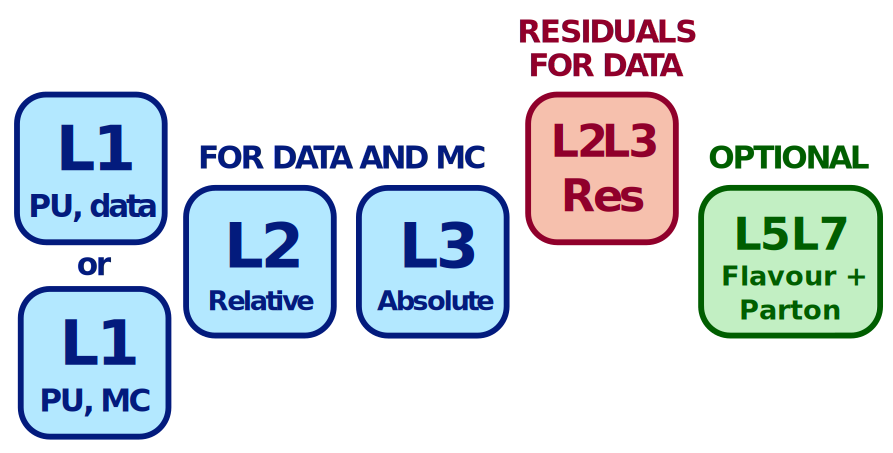
\includegraphics[width = 0.6 \textwidth]{Chapters/Chapter3/Figures/JEClevels.pdf}
 \caption{Schematical overview of the factorized approach adopted in CMS for incorporating jet energy calibrations for data and simulation (MC).}
 \label{fig::JEClevels}
\end{figure}
%The factorized approach starts by firstly removing the contribution of pileup events

\begin{myindentpar}
  \begin{description}
    \item[L1 pileup offset correction] \hfill \\
    The first contribution to the factorized correction chain aims to remove the additional energy deposits originating from pileup interactions in order to only maintain the high-$\pT$ scattering. The corresponding correction term is determined purely from simulation and is based on the average difference in transverse momentum between matched jets with and without additional pileup interactions.
    \\
    
    \indPar The offset energy needed to be subtracted from the jet energy is calculated with a \textit{hybrid jet area method}, which uses the effective area of the jets multiplied by the average energy density in the event and represents the softness of the jet activity. The full correction formula used at CMS is:    
    \begin{equation}
     \mathcal{C}_{L1}\left(\pT^{raw}, \eta, A_{j}, \rho \right) = 1 - A_{j} \dfrac{\left\lbrace \rho_{0}(\eta) + \rho . \beta(\eta) . \left[ 1 + \gamma(\eta).\log(\pT^{raw}) \right] \right\rbrace}{\pT^{raw}}
    \end{equation}
    with $\eta$ the jet pseudo-rapidity, $A_{j}$ the jet area and $\rho$ the per-event $\pT$ offset density. 
    The correction factors $\rho_{0}$, $\beta$ and $\gamma$ are determined in bins of $\eta$ by fitting the offset function using uniquely matched reconstructed jets from the with-PU sample and without-PU sample. 
    The correction formula is applied to both simulated and data events such that an additional scale factor should be taken into account in order to incorporate the small discrepancy between data and simulation.
    This scale factor is only applied for data events and is calculated from the PU-offset corrected transverse momenta of the reconstructed jets.
    %Previous studies have indicated a small discrepancy between data and simulation, which needs to be accounted for since the pileup offset correction is determined completely from simulation. Therefore an additional scale factor needs to be applied to data events to ensure that on average the energy of the reconstructed jets corresponds with the generated MC particle jets. This scale factor is multipied with the jets' PU-offset corrected transverse momenta. 
    
    \item[L2L3 Monte Carlo calibration] \hfill \\
    Now that the $\pT$-response of the jets is independent of the pileup, represented by the number of primary vertices, a following correction should be applied to ensure that the energy of the reconstructed jets corresponds - on average - with the generated jets at particle level and to obtain an $\eta^{PF}$-dependent response. This second calibration is again completely simulation-based and is determined by inverting the $\pT^{gen}$ and $\eta^{PF}$ binned response.
    \begin{equation}
     \mathcal{C}_{L2L3}(p_{\rm T, L1}^{PF}) = \dfrac{1}{\left\langle \frac{p_{\rm T, L1}^{PF}}{\pT^{gen}} \right\rangle \left(\pT^{gen}, \eta^{PF} \right)}
    \end{equation}
    The correction factors are derived from a QCD multijet sample for which a jet reconstruction identical to the one used in data is applied.
    
    \item[L2Residual data-based relative ($\eta$-dependent) correction] \hfill \\
    This first data-based calibration, abbreviated to L2Res, aims at removing the residual difference in $\eta^{PF}$-dependence between data and simulation. For this dijet events with one jet contained in the barrel ($\vert \eta \vert$ $<$ $1.3$) are used. This approach allows to correct the $\pT$ response of all jets relative to the response of central jets based on the expected $\pT$ balance between both jets in the event.
        
    \item[L3Residual data-based absolute ($\pT$-dependent) correction] \hfill \\
    After correcting the relative jet energy scale, the absolute jet energy scale should still be determined. This should only be done for central jets since the L2Res calibration ensures that these values can be used outside the barrel safely. 
    The correction factors are determined using $Z+$jet (with $Z$ $\rightarrow$ $\mu^{+}\mu^{-}$ or $e^{+}e^{-}$) and $\gamma+$jet events since this allows to exploit the precise measurement of the $Z$ and $\gamma$ as reference objects.
    \\
    The L3Res correction tackles the two main remaining differences between data and simulation: slightly lower response for data than for simulation and $\pT$-dependency for the ratio of data to simulation response. These two contributions are independent and can thus be factorized as well. The constant scale factor is determined from the very precise $Z$ $\rightarrow$ $\mu^{+} \mu^{-}+$jet events while the $\pT$-dependent correction factors are obtained by combining the response of all different decay channels in a global fit.
  \end{description}
\end{myindentpar}

Each subcorrection in this factorized approach has specific JES uncertainties which are combined into a systematic uncertainty used in physics analyses. The overall uncertainty is obtained by quadratically adding the uncertainties of each level and is dominated by the $\pT$-dependent difference in pileup offset between data and simulation, the uncertainty of the jet $\pT$ resolution and the lepton/photon scale uncertainties for the L1, L2Res and L3Res subcorrection, respectively.

\subsubsection*{Jet energy resolutions}
Besides the jet energy scale also the transverse momentum or energy resolution (JER) can be influenced by discrepancies between data and simulation. %(\textit{\textbf{Nothing here about difference wrt original configuration?}})
The measurement of the JER is performed using similar methods as applied for determining the JES, but instead of looking at the mean of the response distribution the width is considered.
The jet $\pT$ resolution is determined using QCD dijet and $\gamma+$jet events and results in an $\eta$-dependent data/MC scale factor exceeding unity~\cite{}. Hence the $\pT$ resolution is about $10 \%$ worse for data than for simulation in the barrel, a value which quickly raises to roughly $25\%$ -on average- in the endcap. In order to account for this difference, the resolution for simulation events is worsened by smearing the energy of the corrected PF jets.

\subsubsection*{Identification of b-quark jets}

Identifying the jets originating from b-quark decays consists of constructing observables in order to exploit the differences between b-quark jets and light jets. The algorithms developed for this purpose, many exist in literature, are capable of distinghuishing the event topology of interest from the large bulk of background events which only contain light-parton jets.
The different b-jet-identification or b-tagging algorithms rely on the reconstructed objects defined above although some minor optimization requirements are implied for the track selection to improve efficiency~\cite{}.
\\
One of the main b-quark jet characteristics is the relatively long lifetime of the b-hadron resulting in the presence of a displaced vertex with respect to the interaction point. Since only the tracking detectors offer the spatial resolution needed to detect the displacement between the primary and secondary vertices, they are reconstructed purely from the track collection. In order to be able to cope with multiple proton-proton interactions the tracks are required to be within a cone of $\Delta R$ $=$ $0.3$ around the jet axis, defined by the direction of the jet momentum. 
The actual reconstruction of secondary vertices is an iterative process using an adaptive vertex fit. This fit algorithm estimates the position of the vertex candidate and removes all its associated tracks from the track collection. This fit procedure is repeated until no new vertex candidates can be found. During the first iteration the interaction point is used as a constraint in order to identify the prompt\footnote{Prompt tracks are tracks originating near the pp interaction point.} tracks.

The different b-tagging algorithms existing today can be divided into two distinct categories; one which distinghuishes b-quark jets from light jets based on the track impact parameters and another based on the secondary vertices. Within this thesis only the second type of b-tagging algorithms will be considered, namely the \textit{Combined Secondary Vertex} (CSV) algorithm~\cite{}. This algorithm combines the secondary vertex information with the track-based lifetime properties. Because both characteristics are combined the algorithm is also capable of discriminating between b-quark and light-parton jets when no secondary vertex was reconstructed. In such a configuration the reduced track constraints sometimes give rise to a pseudo-vertex.
\\
The b-tagging algorithms are constructed in such a way that they should only be applied for three predefined operating points which correspond to a specific misidentification probability for light partons of roughly $10 \%$, $1 \%$ and $0.1 \%$ for an average jet $\pT$ of about $80$ $\GeV$ defined respectively as \textit{Loose}, \textit{Medium} and \textit{Tight}. In this analysis only the Tight operating point is considered (\textit{\textcolor{red}{Need to determine the efficiency percentages from the ttbar sample}})

\subsection{Missing transverse energy}\label{subsec::MET}

The vast majority of physical objects produced in particle collisions can be reconstructed from the collection of energy deposits. 
However neutrinos are the exception to the rule since they are weakly interacting and carry neutral charge. Therefore they will traverse the entire detector and escape detection rendering an accurate reconstruction rather challenging.
\\
So in order to ensure the reconstruction of neutrinos or other hypothetical neutral weakly interacting particles, a signal extremely important for many physics analyses, a specific work-around is applied which is based on indirect observations rather than direct measurements. The solution lies to a great extent in the geometrical characteristics of the particle detectors, by requiring them to be hermeticaly closed such that all other particles are propertly detected and cannot leave the detector unseen.
Thus the missing transverse momentum, which corresponds to all neutrinos and other weakly interacting neutral particles present in the event, can be defined from the total transverse momentum of all observed final-state particles~\cite{}. This procedure allows to exploit the high reconstruction efficiency of the particle-flow algorithm for the neutrino reconstruction.
\begin{equation}
 \vecmet = - \sum \vec{\pT}
\end{equation}
\textit{Calibration of $\met$}
%\textit{Some information about $\met$ resolution}\\
%\textit{Which corrections are applied ?}\\
%\textit{For which reason is $\met$ used ?}

%%\dropchapter{0.4in}
\chapter{title} \label{chp:labelTitle}
%\epigraphhead[70]{\epigraph{\textit{If I could remember the names of all these particles, I'd be a botanist.}}{Enrico Fermi}}
%\undodrop

%\include{chapter5/chapter5}
%\include{chapter6/chapter6}
%\include{chapter7/chapter7}
%\include{chapter8/chapter8}

%Appendix
%\appendix
%\chapter{First Appendix}
\section{some section}


\backmatter

% references
\cleardoublepage
\phantomsection
\addcontentsline{toc}{chapter}{Bibliography}
%\bibliography{references}                                           %Why error for the moment?
%\bibliographystyle{lucas_unsrt} % The CMS publication style
%\bibliographystyle{bibstyle}

% the summary
\cleardoublepage
\phantomsection
\addcontentsline{toc}{chapter}{Summary}
%\chapter*{Summary\markboth{\MakeUppercase{Summary}}{}}

The Large Hadron Collider is the first particle accelerator which is capable of providing an abundant amount of top-quark pair events at record-breaking centre-of-mass energies, allowing for a thorough investigation of physics at the TeV scale.
The data collected by the CMS detector during the 2012 run of the LHC is considered in this thesis and the event signature of interest corresponds to the semi-muonic decay of top-quark pair events.
These events have been used to determine whether the top-quark decay vertex is described purely by a left-handed vector coupling, as predicted by the Standard Model of elementary particle physics, or whether additional couplings occur due to new-physics phenomena. In this thesis the focus was on the estimation of the right-handed tensor coupling, denoted as $\gR$.

The study discussed in this thesis is the first direct measurement of the right-handed anomalous tensor coupling of the top-quark decay vertex.
It has been performed using a Matrix Element method, which is capable of extracting potentially the best estimate of any theoretical parameter from a sample of experimental events.
This advanced analysis technique evaluates each event and calculate a corresponding event probability using a dedicated phase-space integration.
%As a result, applying such a Matrix Element method requires a significant computing time such that 
It has been opted to apply a stringent event selection by for instance exploiting the specific characteristics of the b-quark jets in order to improve the reconstruction efficiency.
Two such jets are expected in top-quark pair events since the top-quark decays almost exclusively into a b-quark and a W-boson. 
%Since this reduces the number of selected events that will be processed by the phase-space integrator the required processing time is also seriously decreased.
%In addition, the number of selected events used in the analysis are reduced implying that also the 

With $19.6 \fbI$ of collision data taken at a centre-of-mass energy of $8 \TeV$ a right-handed tensor coupling value of
\begin{equation}
 \gR = -0.0071 \, \pm \, 0.0083 \, (\textrm{stat.}) \, \pm \, 0.0134  \, (\textrm{syst.}) = -0.0071 \, \pm \, \nonumber 0.0160
\end{equation}
was measured, which is consistent with the prediction of the Standard Model ($\gR$ = 0).
Comparing the obtained result with the currently existing exclusion limits for this right-handed tensor coupling also indicates an excellent agreement.
Hence it can be concluded that the Matrix Element method has been successfully applied on the reconstructed collision events recorded by the CMS experiment and has resulted in a rather accurate and first direct measurement of this anomalous coupling coefficient $\gR$.

% resume in dutch
\cleardoublepage
\phantomsection
\addcontentsline{toc}{chapter}{Samenvatting}
%\chapter*{Samenvatting\markboth{\MakeUppercase{Samenvatting}}{}}

{\Large{\bf Titel vertaling}}\\






% acknowledgments
\cleardoublepage
\phantomsection
\addcontentsline{toc}{chapter}{Acknowledgements}
%\chapter*{Acknowledgements\markboth{\MakeUppercase{Acknowledgements}}{}}





\cleardoublepage

%\end{linenumbers}
\end{document}